% The Thesis Introduction
% Lit review, rationale, permission from copyright holder for figs if unchanged, all should be modified, should close with statement of aims to be addressed
\graphicspath{{chapters/1.Introduction/figures/}}

\begin{savequote}[75mm]
Hofstadter's Law: It always takes longer than you expect, even when you take into account Hofstadter's law
\qauthor{- Douglas Hofstadter: \textit{G\"odel, Escher, Bach: An Eternal Golden Braid, 1979}}
\end{savequote}

\chapter{Introduction}

%Diversity of endosymbiosis - its a lot of things, complex, ununified, lots of research
% most prevalent examples shape the eukaroytes - plastids and mitochondria
% hard to study as things have been fixed
%Paramecium biology
%Chlorella biology
%Knowledge of their interaction

\section{Endosymbiosis}

\subsection{What is endosymbiosis?}

Endosymbiosis has proven one of the most fundamental processes in the evolution of the
eukaryotic cell. This process has both shaped the global climate and
created the cellular context in which specialised multicellular organisms have evolved.
% Not sure I like as biofilms etc are arguably complex multicellular organisms

Endosymbiosis is a special case of symbiosis, which in turn is a long-term stable interdependent 
living together (``sym/σύν'' -- together, ``bios/βίωσις'' -- living) of two or more 
organisms to a point of mutual benefit \citep{DeBary1869,Pound1893} (although many now expand 
this definition beyond mutualism to include other categories of biological interactions \citep{Leung2008,OMalley2015}).
What differentiates endosymbiosis from symbiosis in general is that one partner (the endosymbiont) lives wholly
inside (``endo/ἔνδον'' - inside) of another (the host). This ``inside'' can refer to symbionts within intracellular
spaces or in tissues of multicelluar organisms but excludes niches such as the digestive tract of metazoa as 
as this can be considered as an external surface of the host. These latter symbionts are occasionally termed ectosymbionts.
\begin{table}[h]
    \begin{tabular}{@{}cc@{}}
        \toprule
        \multicolumn{1}{r}{\textbf{Interaction Name}} & \multicolumn{1}{l}{\textbf{Interaction Outcome}} \\ 
        \midrule
        \multicolumn{1}{|c|}{Mutualism}               & \multicolumn{1}{c|}{(+, +)}                      \\
        \multicolumn{1}{|c|}{Antagonism}              & \multicolumn{1}{c|}{(+, -)}                      \\
        \multicolumn{1}{|c|}{Competition}             & \multicolumn{1}{c|}{(-, -)}                      \\
        \multicolumn{1}{|c|}{Commensalism}            & \multicolumn{1}{c|}{(+, 0)}                      \\
        \multicolumn{1}{|c|}{Amensalism}              & \multicolumn{1}{c|}{(-, 0)}                      \\
        \multicolumn{1}{|c|}{Neutralism}              & \multicolumn{1}{c|}{(0, 0)}                      \\ 
        \bottomrule
    \end{tabular}
    \caption{An overview of the categories of biological interaction and the effect they have on the two interacting
        biological units, which may be anything from individual species to whole populations. The outcome column 
        contains a tuple relating the effect an interaction has on a pair of interacting biological units. 
        This ``effect'' is often assessed in terms of metrics such as individual fitness, population size and/or
        growth rate.
        Note: parasitism and predation are mechanisms by which an antagonistic interaction may take place \citep{Abrams1987}
        in the same sense that endosymbiosis is a mechanism by which a mutualistic interaction can take place.
        In reality most interactions will not fall neatly into one of these categories and throughout the duration
        of the interaction may display effects which could be described under multiple categories \citep{Leung2008}}. 
    \label{table:biointeractions}
\end{table}

There is a considerable range of different endosymbiotic relationships in nature. They display variation in the 
degree of host-symbiont integration, interdependence and ecological interaction type (see \ref{table:biointeractions}.  
Even if we restrict ourselves to endosymbioses that are largely ``mutualistic'' (noting that the exact nature of
a certain endosymbiosis is highly dependent on the exact ecological context at a particular point of time and doesn't
always neatly quantize \citep{Leung2008})\footnote{Even as early as this we 
    must address a common motif of modern biology: discrete schemas are frequently 
    overlaid on inherently continuous distributions.  These biological quantizations are prone to error (fuzzy delineations)
    and are constantly challenged by novel discoveries which exhibit a mosaic of category features.  
    There are a plethora of examples of this including classification of 
    mitochondria-related organelles \citep{Maguire2014}, types of biological interactions 
    (see \ref{table:biointeractions}), and discussions of the species concept \citep{DeQueiroz2007,Boenigk2012}.
    This is not say biological quantization is without utility or is a futile task.  Indeed, as long as there is a clarity to 
    the application and synthesis these schema then they form a critical (epistemological) framework upon which further 
    research and communication can build. 
    However, care must be taken not to forget that these schema do not reflect reality and can inadvertently obscure
    to the grey areas \citep{Leung2008}.  We also must ensure that the schema used are in concordance with the practalities of the 
discussion at hand (generalising on \citep{Boenigk2012}).}) there is considerable variety.

For example, the degree to which each partner is reliant upon the other ranges greatly. 
A spectrum can be drawn with ``incidental'' endosymbioses such as when a pathogen
escapes digestion by a macrophage at one extreme through facultative interactions where each partner is
capable of, and does, live aposymbiotically for extended life phases. An example of this would be the relationship of
Rhizobia bacteria and legume (Fabaceaea) plants in which the former reduces atmospheric \(N_{2}\) to ammonia (in turn
assimilated into amino acids) \citep{Hirsch1992} in exchange for host derived carbon sources (typically malate 
and succinate) \citep{Prell2006} at a rate of approximately \(5-10g\) C per \(1g\) N 
fixed \citep{Phillips1980} in carefully controlled specialised root nodule structures \citep{Crespi2008}.
On the other end of the spectrum, there are endosymbioses where the distinction between the two organisms is 
all but lost and arguably two distinct evolutionary lineages have become a single unit of selection 
e.g. the bioenergetic eukaryote organelles the mitochondria and the chloroplast. 

Equally, there is a broad diversity in the degree of host-symbiont integration. This is principally in terms of
metabolic connectivity (direct connections between biosynthetic and other metabolic pathways betwee partners) \citep{Karkar2015},
lifecycle integration, and genomic integration (transfer and/or incorporation of genetic material 
between partners) \citep{Timmis2004} (although all categories overlap).

\begin{figure}[h!]
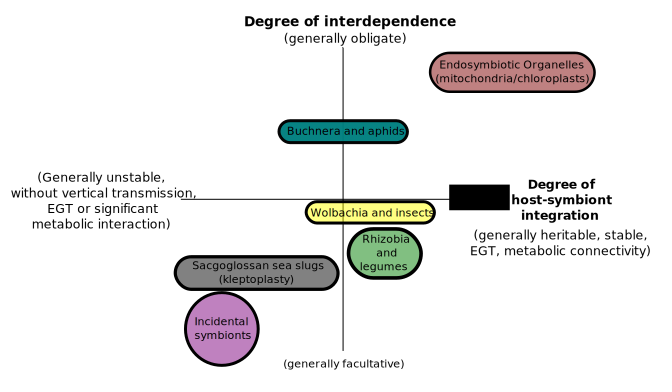
\includegraphics[width=\textwidth]{integration_vs_dependence.pdf}
    \caption{ 
        %%Sacoglossan sea slugs aren't really secondard endosymbionts as they only keep plastid of algea \citep{Christa2014}
        %%NEEDS WORK AS A FIGURE AND CITATIONS FOR CAPTION
        Plot demonstrating a fragment of the diversity of endosymbioses and specifically hilighting the possibility of
        a well integrated by facultative endosymbiosis.
        Host-symbiont integration is a rough measure of how connected the host and symbiont have become genomically, metabolomically
        and in terms of life history.  Whereas, interdependence is a approximate measure of the degree to 
        which the relationship is necessary for life of organisms involved. 
        It should be noted that both axes can be highly reliant on specific ecological and environmental context.
    }
    \label{fig:integrationvsdependence}
\end{figure}

Intracellular endosymbionts can be found inhabiting multiple host-compartments from nakedly in the cytoplasm, to host-derived
vacuolar compartments (often from secretory and endocytic systems) (e.g. \citep{Kodama2009}) along with a range of 
host oraganelles including the endoplasmic reticulum \citep{Vogt1992}, golgi body \citep{Cho2011},
mitochondria \cite{Sassera2006}, chloroplast \citep{Wilcox1986} as well as the nucleus 
(first discovered in \textit{Paramecium} \citep{Schulz2015}).
Owing to the endosymbiotic origin of the chloroplast and mitochdonria (as I will go on to discuss) it becomes apparent
that there can be multiple ``layers'' of endosymbiosis. A primary endosymbiont is an endosymbiont that is the direct
endosymbiont of the host (e.g. the mitochondria to eukaryotes) whereas a secondary endosymbiont is the endosymbiont of
an endosymbiont.
The layers of endosymbioses can get impressively deep, for example, bacterial endosymbionts have been identified within the 
chloroplast stroma (cyanobacterial endosybmiont) of dinoflagellates (e.g. \textit{Woloszynskia pascheri} \citep{Wilcox1986})
In turn, dinoflagellate plastids have been discovered that are likely the product of tertiary endosymbioses \citep{Gabrielsen2011} 
with higher-order events hypothesised in related groups \citep{Stiller2014}.
Therefore, bacteria like this could be the endosymbiont of an endosymbiont of an endosymbiont of an endosymbiont (quatenary) or
higher.

With this considerable diversity it is perhaps not surprising that endosymbioses have been discovered featuring partners from all 3 domains of celullar life. %side-steppin the ole viruses thing 
However, with the exception of one extant Bacteria-Bacteria endosymbiosis \citep{vonDohlen2001}, typically the majority of known
endosymbioses feature a eukaryotic host\footnote{There are however many examples of mutualistic symbioses which are Bacteria-Bacteria (e.g. biofilms \citep{Watnick2000}),
    Bacteria-Archaea (e.g. anaerobic methanotrophic archaea and sulphate-reducing bacteria likely responsible
    for a large proportion of global methane consumption \citep{Boetius2000,Knittel2009} and SM1 
    euryarchaea/\textit{Thiothrix} sp. sulphide-oxidising bacteria \citep{Henneberger2006,Wrede2012}), 
    and at least one example of Archaea-Archaea (\textit{Igniococcus hospitalis/Nanoarchaeum equitans} \citep{Huber2002}. 
    Interestingly \textit{Igniococcus} is the first identified case of an energised outer-membrane in 
    double-membrane bound archaea or bacteria, a significant finding for the development of theories of
eukaryogenesis \citep{Kuper2010})} but can include endosymbionts from all 3 domains.
For example:\footnote{Although with all these example, it is important not 
    to consider an endosymbiotic relationship 
    in isolation from other endosymbionts present in the same host.
    There are examples where facultative ``secondary endosymbionts'' 
    are able to compensate for the loss of an obligate endosymbiont \citep{Koga2003}.  Symbiont-symbiont 
    interactions have been found to play a role in determining which endosymbionts are capable of establishing themselves 
    in a certain host and can even be capable of generating additional phenotypes e.g. the R-bodies of ``killer'' \textit{Paramecium} 
    species which may be a product of an interaction between the \textit{Paramecium} host, \textit{Caedibacter} and a bacteriophage
    \citep{Schrallhammer2009}. %Hydra system is another example}
}
\begin{itemize}
    \item Eukaryote-Archaea \citep{Moissl-Eichinger2011}
    \begin{itemize}
        \item Methanogenic archaea within various ciliates species (e.g. \textit{Plagioplya frontata}) \citep{Fenchel1992,Lange2005}
        \item \textit{Cenarchaeaum symbiosum} within the tissues of marine sponges \citep{Preston1996,Wrede2012}
    \end{itemize}
        \item Eukaryote-Bacteria 
    \begin{itemize}
         \item \textit{Hartmannella} and it's intranuclear endosymbiont \textit{Candidatus Nucleicultrix amoebiphilia} \citep{Schulz2014}
         \item the most famous pairing of mitochondria and plastids
    \end{itemize}
    \item Eukaryote-Eukaryote
    \begin{itemize}
        \item The fungi \textit{Diplodia mutila} which aids heribovery resistance in the palm \textit{Iriartea deltoidea} in lowlight
            conditions but becomes pathogenic if host is well lit \citep{Alvarez-Loayza2011}
        \item Red alga dervied plastids in brown algae \citep{Dorrell2011}
        \item Numerous examples of algal mediated acquired phototrophy in ciliates \citep{Johnson2011}
    \end{itemize}
\end{itemize}

Endosymbiosis is the one of the most significant evolutionary processes in eukaryotic cell.
It offers a means for eukaryotes to benefit from the extensive metabolic diversity
present in the bacterial and archael pangenome, especially the only known forms of primary energy
production - photosynthesis and chemosynthesis \citep{Wernegreen2012}.

It can be argued that endosymbiosis is the process that created the eukaryotic cell and is indeed a fundamental
aspect of eukaryogeneisis.

\subsection{Endosymbiosis and Eukaryogenisis}

%Recombination via transduction, conjugation and/or transformation as found in the bacteria and archaea is
%qualitatively different from that of recombination by sex found in the eukaryotes. 
%Typically, the former leads to the generation of a pan-genome whereas the latter promotes vertical inheritance. \citep{Ku2015}

Every known eukaryotic cell harbours at least 1 endosymbiont in the form of the mitochondria (or a highly
reduced mitochondria-related organelle (MRO)). 

Furthermore, the chloroplast found across every major branch of the eukaryotic tree of life (eTOL)
which facilitates the fundamental process of photosynthesis.





%What is endosymbiosis?
%What are organelles?
%What do we know about the processes by which it has occurred?
%What differentiates organelles and endosymbionts if anything?


Separating organelle and endosymbiont - hard \citep{Keeling2008} Nowack paulinella dispatch

Inherent difficulty of applying a schema of discrete caterogies onto a continuous non-linear distribution



The most prevalent example of this interaction is that of the mitochodria and chloroplasts 
within the eukaryotes.

The most prevalent examples, the chloroplasts and mitochondria of photosynthetic eukaryotes and 
eukaryotes in general respectively, have become obligately dependent on one another to the point where distinguishing 
the two partners as distinct organisms becomes difficult.
With such difficulty distinguishing between endosymbiotic partners it is no 
surprise that the discovery and study of endosymbiosis is relatively recent in 
biology. 



Eukaryote big bang after acquisition of mitochdonria - LECA Pihlippe2000 Koonin2007 - exact time and place and role unknown
Mitochdonria post FECA pre-LECA or Mitochdonria as FECA

Mithcondira first hypothesis - Lane and Martin 2010 bioenergetic explanation




Thus far, I have only discussed primary endosymbioses, secondary yada yada







\subsection{History of Endosymbiosis}

The development of a formal endosymbiotic theory for organellar origin was a process that
lasted 84 years. From, a first tentative mention in a 19th century footnote\footnote{``Sollte es sich definitiv best\"atigen, dass die Plastiden in den 
Eizellen nicht neu gebildet werden, so w\"urde ihre Beziehung zu dem sie 
enthaltenden Organismus einigermaassen an eine Symbiose erinnern. M\"oglicherweise
verdanken die gr\"unen Pflanzen wirklich einer Vereinigung eines farblosen Organismus
mit einem von Chlorophyll gleichm\"assig tingirten ihren Ursprung\ldots''
\citep{Schimper1883} or to approximately translate: ``Should it be confirmed
that plastids are not formed \textit{de novo} in oocytes, their relationship with
their host could somewhat be considered as a symbiosis.  Possibly green plants owe
their origin to a union of a colourless organism and a chlorophyll tinged one.''
\citep{Neuhauser2014}. Interestingly, this paper also coined the term ``chloroplast'' \citep{Sapp2002}} 
where Andreas Schimper considered the potential origin of plants by a symbiotic union. 


to theory of symbiogenisis of Constantin Mereschkowsky (Константи́н Серге́евич Мережко́вский)\footnote{As 
    an aside Mereschkowsky personally strikes a disturbing, having
    collaborated with the Czar's secret police reporting ``dangerous''
    Jews and other ``traitors'' in academia, leading a right-wing nationalist
    and anti-semitic organisation in Kazan, promoting the genocide of the Jews
    (pre-empting the Nazi concentration camps by 13 years) as well as numerous suspected and 
    confirmed acts of paedophilia (including the rape of 26 girls as young as 6 
    (earning him the moniker as the ``Marquis de Sade of Kazan'')).  
    He even authored a novel presenting a paedophilic eugenic-fascist
    society as a utopia.  
    \citep{Sapp2002}.}

22 years later that plastids were once independent photosynthetic bacteria 
(``\textit{Cyanophyceae}'' approximately equivalent to the contemporary Cyanobacteria) 
supported by his and others earlier research on lichens\footnote{Interestingly, 
    there were several early antropomorphic socio-political 
    interpretations of symbiosis in lichens with metaphors ranging from ``communistic'' 
    (Herbert Spencer), ``slavery'' (Simon Schwendener - the discoverer of lichens as
    super-organisms), and ``consortia'' (Johannes Reinke) \citep{Sapp2002}.}
, his work on diatom chloroplast structure, and the discovery of 
photosynthetic ``infusoria'' \citep{Mereschkowsky1905,Martin1999a,Sapp2002}. 

Ivan Wallin extended Mereschkowsky's theories to the idea of that the mitochondria
of the eukaryotes likely originated as another cellular organelle \citep{Wallin1922} 
on the basis of earlier work by Paul Portier attemping to independently
culture mitochondria \citep{Sapp2002} (interestingly, 
Mereschkowsky had strongly refuted this idea just a couple of years earlier as 
an idea that would ruin his ``theory of symbiogenisis'' \citep{Sapp2002} but 
had elaborately comitted suicide the year prior to Wallin's publication \citep{Sapp2002}).

However, these theories never truly reached mainstream acceptance at the time
partially due to the repeated failures to generate direct evidence that mitochondria
and chloroplasts were indeed once free-living bacteria by means of separating them
and culturing them independently from their host cells.  Wallin, Portier, and Faministyn
among other all attempted this but while some success was had by Faministyn
culturing green algae from amoeba, invertebrate hosts all 3 consistently failed
to robustly separate culture either mitochondria or chloroplasts and subsequently
faced moderate to extreme scorn academically \citep{Archibald2014}.
Furthermore, as conceptual and experimental breakthroughs occurred at increasing
rate throughout C20, symbiotic theory fell increasingly out of favour among
the luminaries of the day e.g. Thomas Hunt Morgan and Edmund Beecher Wilson (the
latter of which was directly challenged by Mereschkowsky in his landmark 1905
paper \citep{Mereschkowsky1905,Martin1999a}, and who in return referred to Mereschkowsky's
theories as ``an entertaining fantasy'' \citep{Wilson1928,Martin1999a}
\citep{Archibald2014}. The loud denunciations of Darwinian theories of evolution
by these researchers, especially front-runners Mereschkowksy and Portier as being
insufficient to explain biological novelty relative to their own theories
regarding the acquisition and inheritance of microbes \citep{Sapp2002} no doubt
contributed to this falling out of favour in the face of ascendent neo-darwinian
modern synthesis.


It wasn't until 45 years later and the definitive work of Lynn Margulis \citep{Sagan1967} 
developed in the light of cutting edge discoveries attributable to the nascent
molecular revoltion of biology. Despite ignorance of the earlier work of these 
``symbiogeneticists'' \citep{Archibald2014} Margulis presented 


One of Margulis key innovations was a recognition of the need to expand the
work being conducted in eukaryotic genetic beyond just that of the nucleus
\citep{Archibald2012}.




\subsection{Studying endosymbiosis}



As Kwang Jeon demonstrated host-symbiont co-dependence \citep{Jeon1972} can become fixed in as little as 18 months (200 generations approximately)  \citep{Jeon1978}

However, there are still many open questions in the process of endosymbiosis,
why do the two major facultative endosymbiotic events in the evolution of the eukaryotes
appear to have only occurred once? By what process does endosymbiosis occur?
Why are secondary photosynthetic endosymbioses relatively common?
Unfortunately, these questions are very difficult to answer as in the most successful
and abundant examples metabolic co-dependence between host and endosymbiont has become
fixed.  This limits the abilities of researchers to investigate the nature of the
relationship between host and endosymbiont and thus attempt to answer questions
such as the above. 

However,  





%%%DIFF STUDYING ENDOSYMBIOSIS
% metabolic co-dependence has become fixed
% Kwang Jeon experimental induction  in ameoba 1976-1980 
% there is a need for mocrobial model systems to learn about endosymbioese as they occur so they can be manipulated
% cotinuing a long tradition \citep{OMalley2015}
% still difficult to say how generelazable to the past ARCHIBALDBOOK

However, despite the importance of this evolutionary process there is a relative
paucity of models in which researchers can dissect the mechanisms by which it occur
in\-situ before metabolic co-dependence becomes fixed.














While there was some earlier evidence as to the presence of nucleic acids in 
plastids such as the work by Stocking and Gifford Jr., who demonstrated that
radio-labelled thymidine was incorporated into the chloroplast of \textit{Spirogyra}
\citep{Stocking1959}.
The unequivocable identification of DNA within chloroplasts came via the 
the cytochemical and electron microscopy investigation of \textit{Chlaymdomonas moewusii} 
by Ris \& Plaut \citep{Ris1962} and the subsequent work by direct isolation of
dsDNA from \textit{Chlorella ellipsoidea}, \textit{Chlamydomonas reinhardtii}, spinach
and beet leaves by Chun \textit{et al.} \citep{Chun1963}. The role played by
\textit{Chlorella} here, once again, places it firmly at the roots of endosymbiotic
theory and research.






Margulis' theory was ultimately validated by later work such as that presented in 
``Origins of prokaryotes, eukaryotes, mitochondria, and chloroplasts'' by Margaret Dayhoff 

that proved endosmybiosis \citep{Schwartz1976}










%%%% TRANSITION INTO WHY PHOTOSYNTHETIC ENDOSYMBIOSIS IS SO IMPORTANT
\subsection{Photosynthetic endosymbiosis}

While the acquisition of the mitochondria <++> %when 
is the de facto definitive event in the evolution of the eukaryotic cell, 
it is the later acquistion of photosynthetic organelles (plastid) and the subsequent 
diversification of plants and algae (archaeplastida) that has fundamentally shaped global ecology.

Photosynthesis is the biological process by which energy-rich reduced carbon compounds 
are synthesised from atmospheric \(CO_{2}\) using captured light energy. 
It is a specialised form of phototrophy, in which an organism is capable of trapping
and utilising light energy using photopigments such as chlorophyll, carotenoids, phycobilins
and retinal, flavins and bilins. 
Photosynthesis, releases oxygen as a by-product of using water a the terminal electron receptor 
(however, some bacteria, e.g. purple non-sulphur bacteria and green sulphur bacteria, use alternative
receptors and are thus said to conduct anoxygenic photosynthesis).

There are two stages to photosynthesis, consisting of light-dependent and light-independent reactions respectively.
c3, c4, CAM


As a process, photosynthesis likely predates the eukaryotes with stromatolites microfossils 
indicating the presence of photosynthetic cyanbobacteria like organisms at least 3.5gya.




%two open qs in photosynth endo is which cyanobacteria is the plastid closest to, when did it happen









This is due to photosynthetic organisms (eukaryote and bacteria) forming the basal 
link in almost every major global ecosystem where they act by converting solar energy 
directly into the net primary productivity upon which all other organisms 
deride sustenance \citep{Reyes-Prieto2007}.



Plantes and algae convert approximately 258bn tons of atmospheric \(CO_{2}\) into biomass
annually via photosynthesis \citep{}<++>




The only global ecosystems not reliant on photosynthetic 




The basal position of the plastid bearing branches of the eukaryotic tree of life %GOOD CITATION OF ETOL NOT BALDAUF 2000-2003
suggests the deep seated importance ... something \citep{Yoon2004}


The plastid likely originates from a single ancient primary endosymbiotic event \(\approx 1.6\)gya \citep{Yoon2004}.
This endosymbiosis hypothetically takes place between a photosynthetic bacteria (cyanobacteria) and
an unknown heterotrophic eukaryote \citep{Reyes-Prieto2007}.


Phylogenetic analyses using fossils, cross-calibration, and/or molecular clock estimates indicate 
this took place between \(0.9-1.7gya\) \citep{Yoon2004,Parfrey2011,Shih2013,McFadden2014} and 
suggest that this endosymbiont likely branches basal to cyanobacteria, 



Almost all plastid-encoded genes and endosymbiont genes that have moved to the host's nucleus are 
cyanobacterial in origin 


However, a small but significant subset of genes related to storage polysaccharide metabolism have been 
considered by some researchers to display a separate \textit{Chlamydia}-like evolutionary signature.
This has been cited as evidence of the role of a 3rd party in the primary endosymbiosis which has subsequently
been lost.  However, the lack of present chlamydiales that infect archaeplastida despite broad host-range throughout 
the eukaryotes and re-analysis demonstrating a mosaic of origins for these proteins provides no compelling
evidence for this "menage-a-trois" scenario \citep{Domman2015}.




However, there may be at least one case of an independent primary photosynthetic endosymbiosis, \textit{Paulinella chromatophora}.
\citep{McFadden2014}. \textit{Paulinella} is a euglyphid amoeba with photosynthetic symbionts that bear a much stronger
resemblance to reduced cyanobacteria than the chloroplast of the archaeplastida.  
This is likely more than 60mya  NOWACK2008


Kleptoplastidy in Sacoglossan sea slugs, longevity (months) suggests they are maintained, 
but evidence for endosymbiotic gene transfer in this system is scant (Pierce says maybe2012), Bhatta2013 says no.


There are 3 key stages to ``domestication'' of a photosynthetic endosymbiont: getting photosynthate from it,
procuring genes to supply it with protein, regulating its division \citep{McFadden2014}.

plastidic phosphate translocators (pPTs) occur in all know plastids therefore likely predate divergence so were
likely present in the initial acquisition.  Always antiporters, quid pro quo etc  most important


Plastids have 100-200 genes (\textit{Paulinella} has <++>) from thousands as free-living
Transfer of genes to host has advantages: endosymbionts are clonal in host - no exchange therefore no purifying seleections
Muller's ratchet - mutation accumulation.
Genes in sexual host - diploidy, recomb and purifying.
Minimise oxygen species damage.
Why are 100-200 maintained?
Frequent on reconstructiomn in tobbaoca HUANG2003

"Limited transfer window" hypothesis : hosts with multipel endosymbionts have a higher chance of transfer than hosts 
with one or a few cf. Chlamydomonas to Plants Lister2003 Smith2011. More symbionts = more donrs 
Tranfer of DNA INTO plastids is very rare  

Most EGT will be lost but ones that are transolacted into endosymbiot will be kepts TOC TIC N-terminal signlal: peps
Lock-in dependence on host - selectid for .


Finally division: plastids are vertically inherited - therefore they need to replicate before host division.

Too quick they kill host, too slow they don't work well and won't be abundant enough to go in daughter cells


All divide using FtsZ apart from apicomplexan non-active ones Francia2012
Most pllstid dividion machinery originates from homologous binary fission machinery in cyanobacteria
but some key parts are eukaryotic - suggesting host is controlling 

FtsZ asssembles into Z-ring at plastid equator using Min D,E motor proteins 
This is tethered to inner env membrane with ARC6 (likely euk)
Bunch of crap is recruited, another ring DRP5B (euk origin)- ring also forms on host side of outer plastid membrane (PD)
\citep{McFadden2014}









Subsequently, there appear to have been multiple secondary endosymbioses between plastid-bearing eukaryotes
and other eukaryotes.






Plastids-bearing eukaryotes 






Photosynthetic endosymbiosis has occurred 




1.558gya 
red-green algae split 1.5gya
1.3gya origin second endosymbiosis \citep{Yoon2004}





%STATE OF PHOTOSYNTHETIC ENDOSYMBIOSIS

% Primary likely occurred once but all over the place there are secondard
%endosymbioses

%% With the exception of the primary endosymbioses of the archaeplastida, almost all oxygenic phototrophs are believed to have arisen via secondary or higher order symbioses \citep{Hoshina2009} {}<++>

%plastids all over the place even (INCLUDE OTHERS) rappemonads \citep{Kim2011a}







%%Importance of gene duplication in explaining fungal metabolic diversity compared to
%%HGT however, this is specifically related to gene clusters both GD and HGT more
%%pronounced in clustersA
%%GD dominant and across all taxa, HGT lineage specific innovation
%%The disproportionate effect of GD and HGT on clustered genes renders metabolic gene clusters into hotspots of metabolic innovation and diversification in fungi
%%Intriguingly, earlier diverged fungi had lower numbers of duplicated EC-annotated metabolic genes per genome possibly spurious due to few genomes
%%\begin{math} 2.8\% \end{math}
%%\citep{Wisecaver2014}, different from animal 
%%HOX tandem duplication clusters because they are evolutionarily unrelated
%%but can't tell if there 
%%are clusters in \textit{Paramecium}
%%In archaea and bacteria ``extensive gene loss and horizontal gene transfer leading to innovation are the two dominant evolutionary processes, and yields robust estimates of the supergenome size.''
%%(note that this paper looks at 34 bacterial groups but only 1 archaeal) \citep{Puigbo2014}
%%Recent emergence of ubiquitous bacterial horizontal regulatory transfer 
%%``bacterial genes can rapidly shift between multiple regulatory modes by acquiring functionally divergent nonhomologous promoter regions'' 
%%Same forces that drive coding HGT can also transfer regulatory non-coding regions that can have profound phenotypic consequences \citep{Oren2014}
%%``the ubiquity and extent of HRT have not been appreciated before the study of Oren et al'' \citep{Koonin2014}

%%Eukaryote genome biology is important but very skewed \citep{DelCampo2014}
%%\textit{Paramecium bursaria} 


%%%%``There are numerous features that are specific for eukaryotes and can be traced back to the last 
%%Eukaryotic common ancestor (LECA), such as the nucleus, the endomembrane system62–64, the 
%%Mitochondrion65,66, spliceosomal introns67,68, linear chromosomes with telomeres synthesized by 
%%Telomerases69, meiotic sex70, sterol synthesis71, unique cytokinesis structures72 and the capacity 
%%For phagocytosis'' \citep{Gribaldo2010}



Acquisition of phototrophy does not commit an organism to a phototrophic lifestyle
as can be observed in various the transitions of free-living autotrophic algae 
to obligate parasites.  For example, apicomplexans such as \textit{Plasmodium} 
(causative agent for malaria) are derived from red-algae (secondary plastid).
There are also examples of green algae such as \textit{Helicosporidia} that 
adopt a parasitic lifestyle despite having primary plastids. 
Intriguinly, H. parasiticum doesn't seem to demonstrate the same level of
genome reduction as other paraistes.\citep{Pombert2014}
``within this single lineage are found free-living autotrophs like most
other green algae, but also a variety of symbiotic species,
opportunistic pathogens, and perhaps even obligate intracellular
parasites,''
``but a variety or parasitic lineages
had at one time photosynthetic ancestors, including oomycetes,
several dinoflagellates, and most famously the apicomplexan
parasites such as the malaria parasite, Plasmodium (refs 10-11)
and references therein)''
\citep{Pombert2014}
Plasmodium switched to parasitism over 1bya by some estimates, another example
of difficult to discern processes because all traces have been lost (like symb)



``Molecular clock analyses have esti- mated the origin of the green lineage between 700 and 1500 mya (Douzery et al., 2004; Hedges et al., 2004; Berney and Pawlowski, 2006; Roger and Hug, 2006; Herron et al., 2009)''
\citep{Leliaert2012}
``chlorophyte-streptophyte split at 700-1500Mya with similar refs to leliaert'' \citep{DeWever2009}
Trebouxio somewhere between 500-1000Mya, \citep{DeWever2009}



Says \citep{DeWever2009} indicates chlorellaes 100mya \citep{Pombert2014}

Helicosporidia has nearly all metabolic genes of chrloella and coccomyxa apart from
a few minor components of photosynthesis \citep{Pombert2014} from genome seq(all genes relating to light harvesting andelectron transport are missing)




srrison1945equenced chlorophytes range from  67 64 65 64 59 60 gc percentage \citep{Blanc2010a}

sequenced paramecium genomes ranges from 28.2 25.8 28.0 24.1 gc percentage \citep{McGrath2014}







\section{\textit{Paramecium bursaria}}

\textit{Paramecium} are \(80-150\mu m\) phagotrophic single-celled eukaryotes belonging 
to genetically diverse \citep{Prescott1994} sub-grouping of the alveolates known as the ciliates.
They have been studied since the invention of microscopy (first recorded by a contemporary of van Leeuwenhoek 
(see \ref{fig:huygens}) and as such have a well-developed theoretical literature and several available genomes.  

The ciliates are, as their name suggestes, are covered by cilia. 
These are minute hairlike biochemically heterogeneous organelles capable of sensing the environment and by
beating providing cellular locomotion and, in the case of phagotrophic ciliates like \textit{Paramecium}, forcing food bacteria towards
the oral groove (cytopharynx) where they can be phagocytosed \citep{Hamel2011,AubussonFleury2015}. %no phagocytotic ciliates?
\textit{Paramecium} is also capable of rapid locomotion via the expulsion of trichocysts.
These are defensive membrane-bound organelles known as trichocysts containing a crystalline spike which can be 
rapidly ejected into the environment on fusion of trichocyst membrane with plasma membrane \citep{Hamel2011}.

\begin{figure}[h!]
    \caption{\textbf{A}: Carving of Christiaan Huygens (1629-1695), the prominent Dutch Golden Age mathematician and scientist and contemporary of Antoni van Leeuwenhoek, from a medallion by Jean-Jacques Cl\'erion 1679 (reproduced from \citep{Huygens}). \textbf{B}: Likely the first sketch of the micro-organism that we now know as \textit{Paramecium} by Christiaan Huygens in a letter (No. 2133, 11th of August 1678) to his father Constantijn Huygens. An approximate translation of the accompanying text goes as follows ``I have twice seen in this water an animal 10 times as large as the others and with feet all over its body and a narrow form. 4 or 5 feet stirred even when the animal was at rest. It moves as fast as the others, turning and spinning in the water. Hartfoecker thinks he may have discovered the same species in `semine corrupto' (as a dried out husk?).'' (reproduced from \citep{Huygens}). \textbf{C}: 8 of the 10 volumes of the collected correspondances of Christian Huygens as prepared for the Dutch Society of Sciences and published from 1888-1905)}
    \label{fig:huygens}
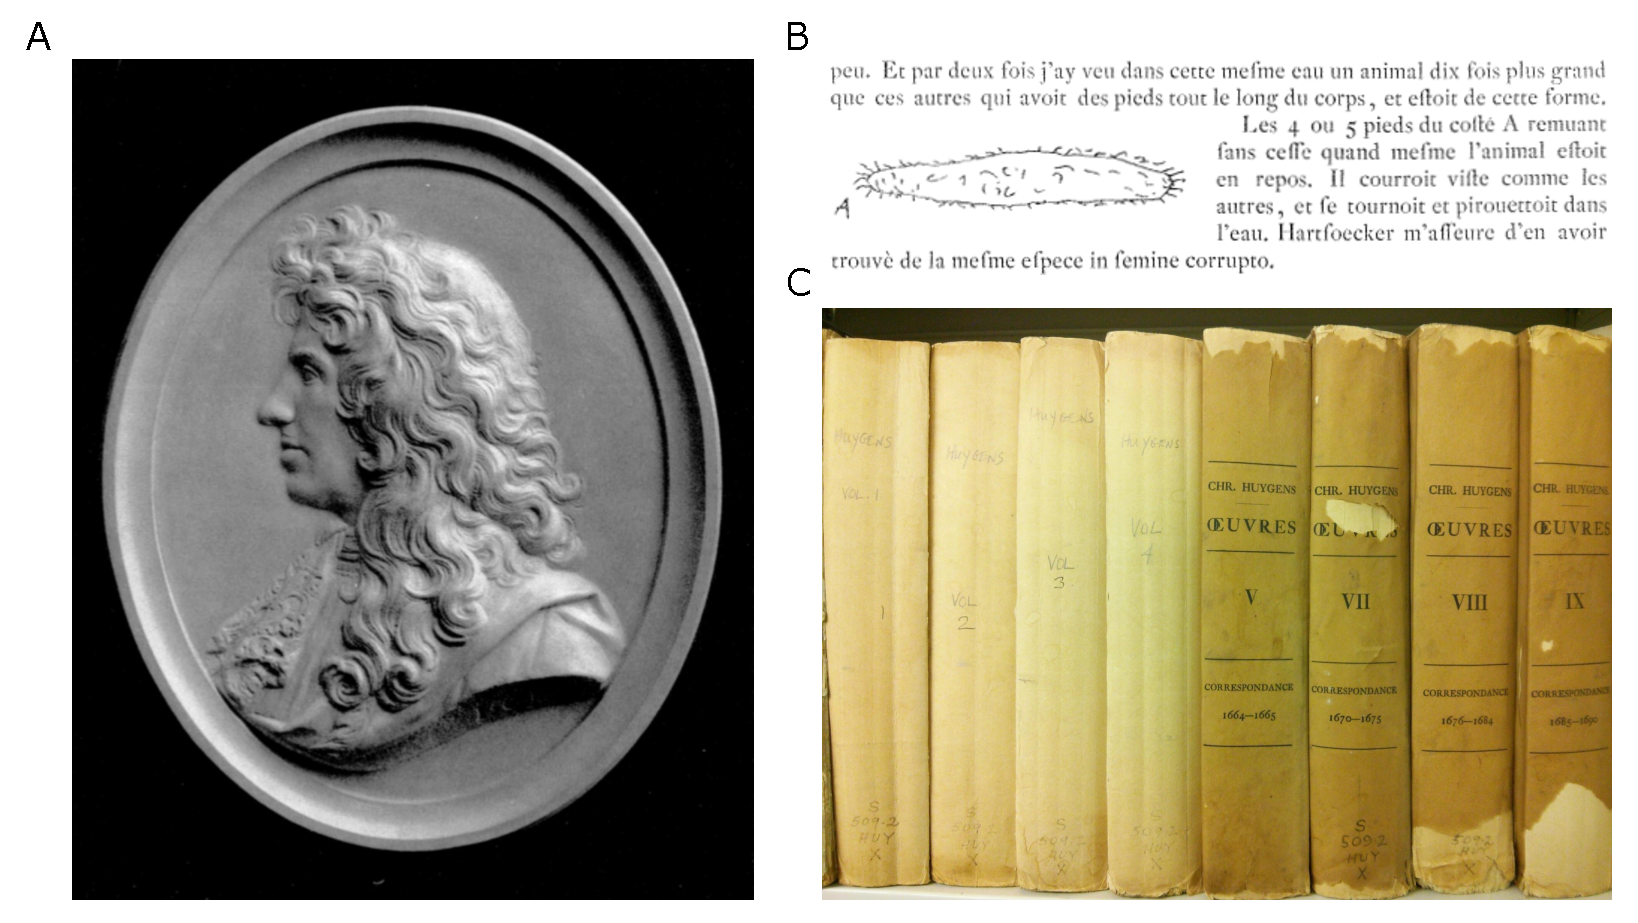
\includegraphics[width=\textwidth]{Christiaan_Huygens_combined_figure.pdf}
\end{figure}

\textit{Paramecium bursaria} ``the green \textit{Paramecium}'' is distinguished from other \textit{Paramecium} by stable, heritable
secondary photosynthetic endosymbiosis it maintains with any of several species of the green algae \textit{Chlorella}.
Each \textit{P. bursaria} cell contains roughly 300 endosymbiotic algae maintained in individual perialgal vacuoles (PV) around the cell
cortex \citep{Hoshina2009}.

\textit{P. bursaria} does share the other distinguishing feature of ciliates: nuclear dimorphism.

\subsection{Nuclear dimorphism}

Ciliates are the only know unicellular group to show germline sequestration away from somatic function in the form of ``nuclear dimorphism'' \citep{Jahn2002}.
Specifically, they have two types of nuclei, expression optimised highly polyploid somatic macronuclei (MAC)
and largely silent diploid germline micronuclei (MIC) \citep{Prescott1994}. 

The exact number of MIC and MAC varies widley by species and genus (\textit{Tetrahymena} has 1:1, 
\textit{Oxytricha trifallax} 1:2-4, and \textit{Paramecium aurelia} 2:1), however, \textit{P. bursaria}
contains a single MIC consiting of 80 to several hundred chromosomes depending
on the exact subspecies \citep{Chen1940}. 

Despite having undergone fewer WGD that \textit{P. aurelia} 

During normal vegetative growth



%considerably larger than that of \textit{Paramecium aurelia} %counter-intuitive with WGDs'



  


MIC DNA is densely packed in chromatin during vegetative growth phases 

The exact number of MIC
varies by species and genus, 

In \textit{Paramecium bursaria} there is 10-30 times the MAC DNA than MIC DNA.  The MIC of \textit{P. bursaria} is 
considerably larger than that of \textit{P. aurelia} \citep{Cullis1972}

Typically, there is a single MIC (of the ``caudatum'' type) with chromosome number and correlated MIC size
varying between 80 and several hundred in different ``races''.  MAC is the same size across ``races'' however.
This variation in the MIC may be a result of multiple pro-nuclei fusing \citep{Chen1940}


Single MIC in each mate meoticially divides wtwice, one produce of each division disintegrates, so only a single
reduced haploid MIC survives. This undergoes mitotic division to produce a male and female gamete.
The male gametes are reciprocally exchanges and fuse with the station female nuclei to form a syncaryon in each conjugant
Each syncaryon divides once and one product disintegrates 
Surviving nucleus divides twice and its 4 produces differentiate into 2 macronuclei and 2 micronuclei
Same time - conjugants split - first cell division restires normal 1mac and mic
\citep{Siegel1963} %based on 

Conjugants don't typically exchange cytoplasm (except under special conditions such as antibody treatments \citep{Harrison1945} .
\citep{Siegel1963}



\textit{Paramecium bursaria} has not naturally been discovered to undergo autogamy \citep{Siegel1963,Yanagi2004} but it can be induced
by treatement of methyl cellulose \citep{Yanagi2004}

Life history - sexual immaturity - transitional period with some sexual - maturity (much sex) - decline


\begin{figure}[h!]
    \caption{\textbf{A}: Carving of Christiaan Huygens (1629-1695), the prominent Dutch Golden Age mathematician and scientist and contemporary of Antoni van Leeuwenhoek, from a medallion by Jean-Jacques Cl\'erion 1679 (reproduced from \citep{Huygens}). \textbf{B}: Likely the first sketch of the micro-organism that we now know as \textit{Paramecium} by Christiaan Huygens in a letter (No. 2133, 11th of August 1678) to his father Constantijn Huygens. An approximate translation of the accompanying text goes as follows ``I have twice seen in this water an animal 10 times as large as the others and with feet all over its body and a narrow form. 4 or 5 feet stirred even when the animal was at rest. It moves as fast as the others, turning and spinning in the water. Hartfoecker thinks he may have discovered the same species in `semine corrupto' (as a dried out husk?).'' (reproduced from \citep{Huygens}). \textbf{C}: 8 of the 10 volumes of the collected correspondances of Christian Huygens as prepared for the Dutch Society of Sciences and published from 1888-1905)}
    \label{fig:huygens}
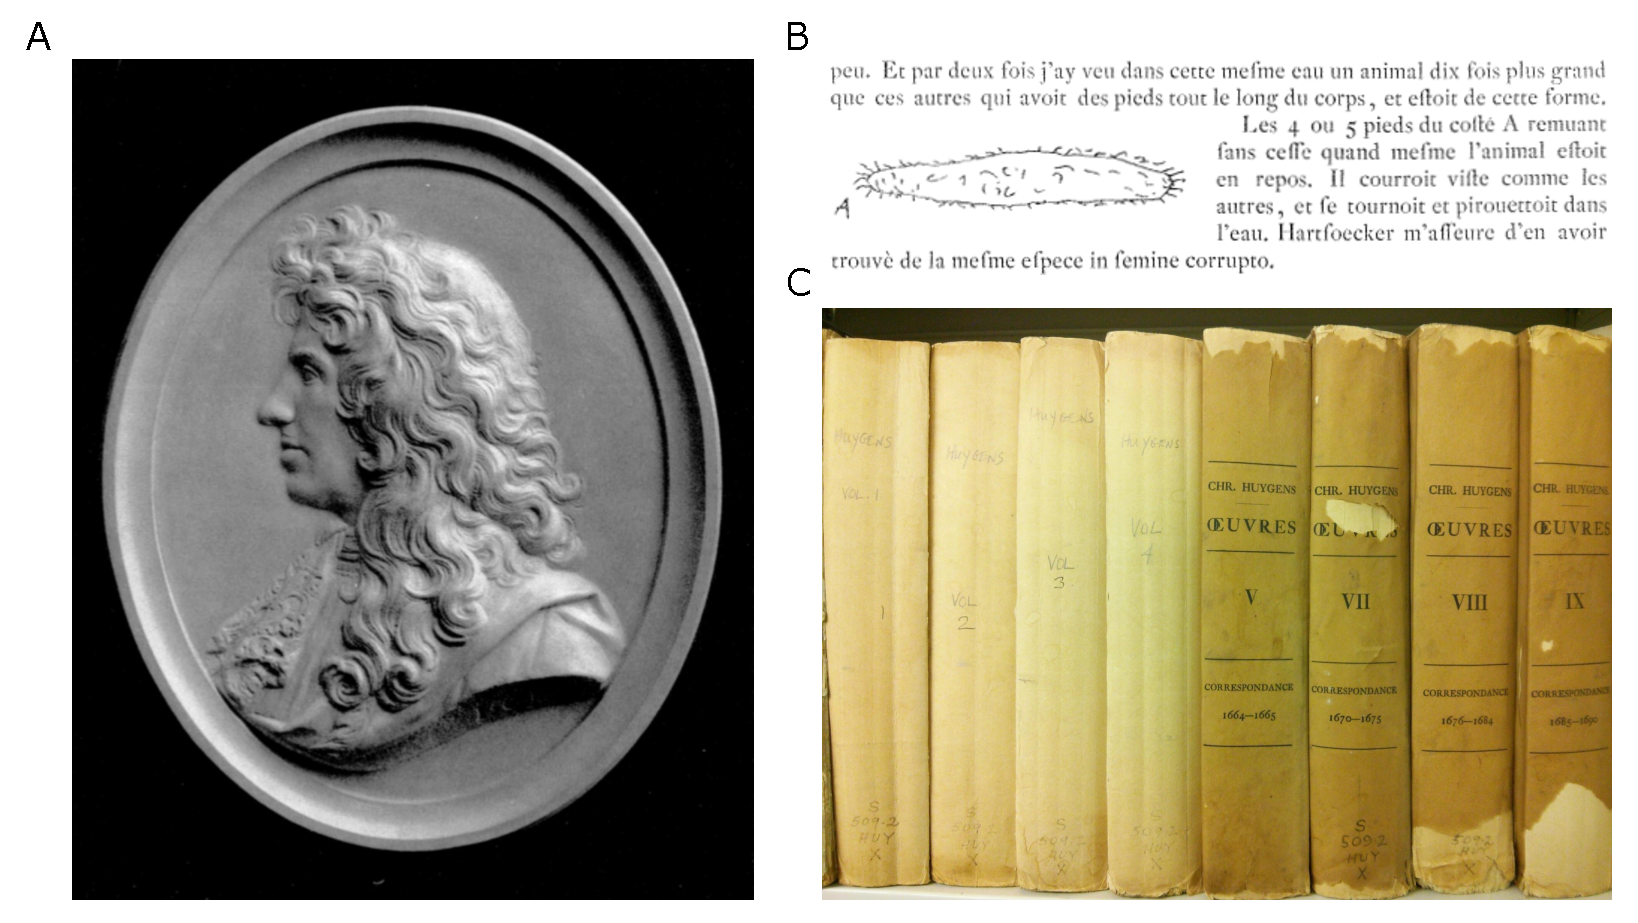
\includegraphics[width=\textwidth]{Christiaan_Huygens_combined_figure.pdf}
\end{figure}




\textit{P. bursaria} is likely to have a MAC genome somewhere between 40 and 100Mb containing somewhere between 
18,000 and 40,000 genes based on the size of the \textit{Tetrahymena} \citep{Eisen2006}, \textit{P. tetaurelia} \citep{Aury2006} and
\textit{Oxytricha} \citep{Swart2013} genomes.











\textit{Paramecium} have received considerable study over the years with (MAC) genome sequencing data
available for 2 strains of \textit{Paramecium tetaurelia} \citep{Aury2006} as well as assemblies for 
\textit{P. caudatum}, \textit{P. multimicronucleatum}, and \textit{P. aurelia} complex species \textit{P. sexaurelia},
\textit{P. primaurelia}, \textit{P. octaurelia} and \textit{P. tredecaurelia} on ParameciumDB (as of 05/03/2015) \citep{Arnaiz2011}.
Furthermore, there are genomes for two relatively closely related ciliate species 
\textit{Tetrahymena thermophila} \citep{Eisen2006} and \textit{Oxytricha trifallax} \citep{Swart2013}.



The \textit{Paramecium tetaurelia} macronuclear genome shows a large (39,642 genes), AT-rich (28\% GC),
mostly repeat free, c
compact (78\% coding density), 
with very small intergenic regions and introns (averages of 352 and 25bp respectively)
No clear evidence of algal ancestry - throwing doubt on the ``chromalevolate'' hypothesis or suggesting total loss
of these features 

WGD  where a large number 51\% of duplicated genes are still present with highly conserved synteny

3WGD  + 1 ancient one

An ancient WGD is likely to have taken place before the divergence of \textit{Tetrahymena} and \textit{Paramecium}
Followed by 2 WGD sometime after the divergence of \textit{Paramecium bursaria}, with a final recent WGD
directly basal to the \textit{P. aurelia} species complex (after the divergence of \textit{P. caudatum} and \textit{P. multimicronucleatum}.
This latter WGD is posited as a potential reason for the speciation in the \textit{P. aurelia} complex 
Paramecium can undergo self-fertiiliisaiton

System for studying the fates of duplicate genes  - high retetion and sytenty 
\citep{Aury2006}

Based on \textit{P. tetaurelia} there appears to be an incredibly high level of replication fidelity and thus low rate of 
base-substitution mutations in these organisms possibly in the same manner as the low observed mutation rate in metazoan germlines
as these mutations are masked until sexual reproduction.  This is probably facilitated by a ciliate specific modifications in the
active sites of B-family polymerases \(\alpha, \zeta\), and the proofreading exonuclease of DNA polymerase \(\epsilon\) \citep{Sung2012}




\citep{Sung2012} or 30-50 when starved \citep{Berger1986} undergo autogamy in which
the old MAC is destroyed and reconstructed from the MIC. 

With compatible mating types it will undergo conjugation.




Ptet after 75 vegetative fissions under high-growth \citep{Sung2012}


Also CpG depressed - normally associated with cytosine methylation but this has not been observed in \textit{Paramecium}
Large numbers of genes with a large number of short introns (Ptet) \citep{Aury2006}




In Ptet
Generating the MAC from the MIC involves 3 steps:
\begin{enumerate}
    \item DNA amplification from diploid to high copy number (approximately 800n in Ptet)
    \item DNA elimination pathway 1 : removal of short unique-copy elements (IES, internal eliminated sequences) that run through coding and non-coding sequences
        IES are bound by 5'-TA-3' dinucelotides and are precisiely excised using
        double-stranded breaka and end-joining leaving only one TA dinucelotide in chromosome (60,000 IES in Ptet)
    \item Imprecise removal of large regions (often with TE) similar to transposon silencing in other eukatytes.
        short ncRNAs liekly targeting heterochromatic formation through histone methylates) heterochromatic in lost during MAC dev
        this causes chromsome framgent often, new chroomosme are healed by addition of telmoeres
\end{enumerate}

While these rearrnagements are highly reproducible they seem to generate some heterogeneity in MAC even in clonal cell populations





\begin{figure}[h!]
    \caption{
        Figure redrawn and modified from \citep{Duret2008}.
        During normal vegetative growth \textit{Paramecium bursaria} (and other \textit{Paramecia}) divide by binary fission with the MAC
        elongating and ``pinching'' off in a process distinct from mitosis (known as amitosis) while the MIC undergoes mitosis.
        As the cell pinches before cytokinesis an unknown septum forms at the ``neck'', this stops cytoplasmic streaming which induces
        the endosymbionts to begin to divide. Cytokinesis then occurs largely simultaneously in host and endosymbionts \citep{Kadono2004,Takahashi2007}.
        The sexual cycle involves conjugation of compatible mating types which triggers two-rounds of meosis of the MIC with
        one product disintegrating after each division so only a single haploid MIC remains. This undergoes mitosis to produce male and
        female gametes. Male gametes are then reciprocally exchanged between mating cells and fuse with the respective female gamete to 
        create a syncaryon. Each syncaryon divides onces and one product disintegrates before undergoing two subsequent divisions.
        Two products differentiate into MACs by programmatic reorganisation, conjugants split and a normal binary fission occurs 
    restoring normal 1 MAC and 1 MIC \citep{Siegel1963} }%based on }

\end{figure}

        with meiosis of the two MIC to yield eight haploid products, seven of which degenerate. The eighth haploid gametic nucleus copies itself by mitosis

        and the two identical haploid nuclei fuse to from a completely homozygous diploid zygotic nucleus. Two post-zygotic mitotic divisions yield four diploid

        germline nuclei, which migrate to positions at the anterior and posterior of the cell. The two nuclei at the cell posterior differentiate into new MACs,

        the two nuclei at the cell anterior are the new MICs. During the first, caryonidal, cell division the macronuclear anlage do not divide. One is distributed

        to each daughter cell as they continue to endoreplicate DNA to attain the final MAC copy number of ∼800 n. After a second cell division in which both

        the MICs and the MAC divide, the sexual progeny enter the vegetative phase. Note that the progressively fragmented maternal MAC is present

        throughout meiosis, fertilization, and MAC differentiation and remains transcriptionally active. The fragments are lost by dilution in the course of the

        first cell divisions. The same events occur during conjugation; however, there is reciprocal exchange of haploid gametic MICs, so that the diploid zygotic

        nucleus produced by fertilization in each conjugating cell is heterozygous at all loci. Both sexual processes can be induced by standard laboratory

        protocols (Sonneborn 1974)
    }
    \label{fig:huygens}
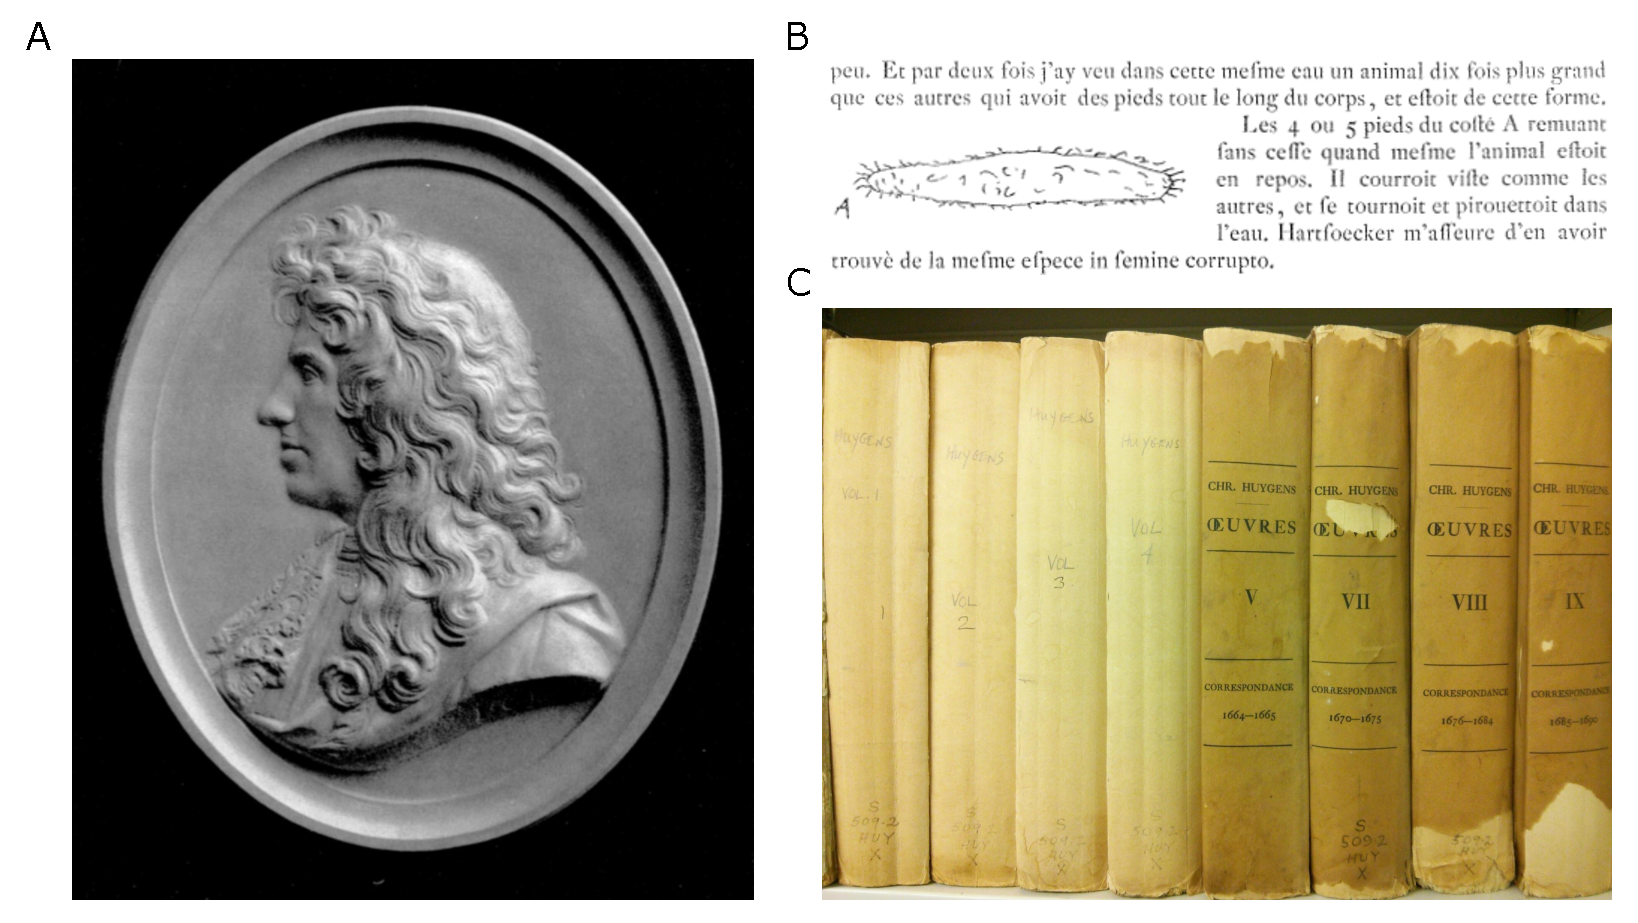
\includegraphics[width=\textwidth]{Christiaan_Huygens_combined_figure.pdf}
\end{figure}










\textit{Paramecium} species have multiple mating type systems \citep{} %Jennings 1938 + Sonneborn papers before 1938

two-locus hypothesis but invoked instability and may require epigenetic and genetic systems \citep{Siegel1960}





\begin{figure}
    \includegraphics[width=\textwidth]{trees_of_life.pdf}
    \caption{\textbf{A}: Schematic of the current best estimate of the tree of life demonstrating the 2D and 3D hypotheses,
dashed lines indicate multiple potential branch location, arrowed lines demonstrate known endosymbiotic events (based on work reviewed in \citep{Gribaldo2010})
\textbf{B}: Schematic of the current known eukaryotic portion of the tree of life (based on work reviewed in \citep{Burki2014,Adl2013},
\textbf{C}: Schematic of phylogeny of the ciliates (based on work by \citep{Bachvaroff2011} showing Oligohymenophorea containing \textit{Paramecium} and \textit{Tetrahymena} and sister group Spriotrichea containing \textit{Euplotes} and \textit{Oxytricha}.
\textbf{D}: Schematic of phylogeny of the green algae (based on work reviewed in \citep{Leliaert2012}
    \label{fig;tol}
\end{figure}





The MAC is lost at each sexual generation
and must be regenerated from the MIC following meiosis \citep{Aury2006}.
This process involves a dramatic genomic rearrangement at a scale largely unprecedented in other studied organisms
outside of terminal somatic differentiation in a range of metazoans \citep{Jahn2002}.




The other characteristic feature of the ciliates is that of being-covered in complexes of cilia (for which they are named) 
used for movement and phagocytotic food capture \citep{Prescott1994}.


Mating in \textit{P. bursaria} 









MAC/MIC ratio varies by species %WHAT IS PB? 1:2 I think...
MIC - mitosis in vegetative - meiosis otherwise
MAC - amitosis "pinching"

This nuclear dimorphism is what allows genomic consistancy to be maintained despite major genomic reorganisation

Large \(100-250\mu m\) 


\textit{Paramecium} has been studied since the origin of microscopy \citep{Gortz2009}


Different genetic code:


in a process that displays
a dramatic genomic rearrangement

MIC consists of over 50 chromsosomes with an uncharacterised centromeric and telomeric structure \citep{Aury2006}.

MAC is generated by 



The macronuclear genome undergoes 




Sequenced ciliate genomes: Oxytricha trifallax, Tetrahymena thermophila, Paramecium biaurelia, tetaurelia, multimicronucleatum
caudatum, sexaurelia, primaurelia



Genetics in the \textit{Paramecium} was some of the founding work on the genetics of unicellular eukaryotes.
Throughout the 50s and 60s almost every genetics textbook addressed it at length 
They demonstrate frequent, complex non-mendelian inheritance e.g. cytoplastmic inheritance of killer phenotyopes, 
But have declined in study today possibly as a product of complexity, death of sonneborn \citep{Preer1997}


Paramecium bursaria micronuclei frequently contains bacterial endosymbionts.  Possibly due to the closed
nature of reproduction endonuclebioses are common in paramecium.  Larger MIC than Aurelia \citep{Gortz2009}



There is no evidence of a plastid or plastid-derived compartment within the ciliates.
There is some evidence of approximately 16 genes of algal origin within the ciliates 
Potentially, these could be the remnants of a lost plastid, in the same way remnants of mitochondrial function 
exist in organisms with highly derived MROs such as \textit{E. histolytica} fitting with the secnario of
secondary loss of a plastid which could be proved by finding an ancestral photosynthetic lineage.
In the same way that plastid bearing \textit{Chromera velia} is touted as evidence for the photosynthetic activity
of an cestral apicomplexans. \citep{Reyes-Prieto2008}



\textit{Paramecium} appears to be particularly competent for endosymbioses with an array of over 60 
genetically diverse endosymbionts described \citep{Gortz2009}.

Ciliates in general are known to have bacterial \citep{Gortz2009}, archaeal \citep{Wrede2012} and eukaryotic \citep{}<++>





bacterial endosymbionts documented in the literature \citep{Gortz2009}
These endosymbionts range in degree from mutualist to downright parasitic and are cytoplastmic, endomicronucleic,
endomacronucleic and/or perinuclear. 

Some exhibit high levels of adaptation, no longer able to be found free-living and with evidence of the genome reduction
distinctive of endosymbiosis \citep{Gortz2009} %No specific citation in revirw

The most frequently identified bacterial endosymbionts in German environmental samples are that of \textit{Holospora  caryophila},
\textit{Holospora obtusa} and \textit{Caedibacter caryophilus}


Several symbionts of Paramecium have been shown to require the presence of specific Paramecium genes for their maintenance (Sonneborn 1943 ; Schneller et al. 1959 ; Gibson and Beale 1961; Fujishima and Fujita 1985)


As a serial phagotroph, \textit{Paramecium} species are liable to infiltration by bacterial capable of escaping or resisting
the phagosomal digestive process FOK ALLEN 1988 LYOSOEOME SYSTEM IN PARAMECIUM PRINGER BERLIN 301-324






The most famous of these is that of the so-called ``killer endosymbionts'' 


Tracy Sonneborn, the father of modern \textit{Paramecium} research may two key discoveries:
morphologically identical \textit{Paramecium aurelia} strains were unable to mate 

And secondarily there were a plethora of cytoplastmic particles within several paramecium species
that were capable of conveying cytoplastmic inheritance of certain traits.

Laterly these particles are mostly identified as symbionts 


\citep{Corliss1974} 





As mentioned earlier, when one considers the influence Tracey Sonneborn's discovery of non-mendelian
inheritance non-mendelian inheritance in the related \textit{Paramecium (aurelia)}, where he showed
cytoplasmic inheritance of features such as cilia orientation\footnote{``Pieces of cortex of Paramecium can be grafted onto a whole cell and
become integrated, yielding a modified cortical pattern which is maintained through both sexual and asexual reproduction.'' \citep{Beisson1965}}

the development of Margulis' forumaltion of endosymbiosis \citep{Margulis1998} it is
quite appropriate that we are revisiting this organism

Sonneborn's classic review \citep{Sonneborn1950} proved a verdant source of methodologies
for research on  \textit{P. aurelia} and \textit{Paramecium} in general



Generally, \textit{P. bursaria} is marked by its distinctive photosynthetic green algal endosymbionts.
However, can lose them, YSA2 is natural mutant that doesn't maintain them due to breakdown of the mechanism
that partitions endosymbionts between cells at reproduction \citep{Tonooka2002} %good material on algae free in first paragraphs-come back to this paper



%Furthermore, Mereschowsky considered a very similar system to \textit{Paramecium bursaria} and 
%its green algal endosymbionts as a key line of evidence in the development
%of his theory of symbiogenisis (the organism \textit{Amoeba viridis}, now known as
%\textit{Mayorella viridis} \citep{
%\citep{Mereschkowsky1905,Martin1999a}
%Indeed protists containing green algae such as \textit{Paramecium bursaria} referenced
%as ``animals on the way to becoming plants.'' were considered by Мережко́вский 
%as ``\textit{ad oculum} examples of the (endo)symbiotic nature of plants \citep{Mereschkowsky1920,Sapp2002}. 





%%``The story is told that Sir Robert Peel, the Prime Minister, visited Faraday in the laboratory of the Royal Institution soon after the invention of the dynamo.
%%Pointing to this odd machine, he inquired of what use it was. Faraday is said to have replied `I know not, but I wager that one day your government will tax it.'''
%%from \citep{PearceWilliams1965} potentially apocraphyl (it took until 50 or so years after the 1880s for this prophecy to become true)
i

Multiple ciliates have acquired phototrophy \citep{Johnson2011}



Genome sizes: early densitometer studies found that \textit{Paramecium bursaria} syngen 4 
micronuclei consitently contained \[ 7.5*10^{-12}g \] DNA under all culture conditions so 
approximately a haploid micronuclear genome size of \[ 2.25*10^{12}\] daltons.
MAC contains approximately 20 times as much DNA as diploid MIC (ranging from 10-30
depending on cell state).
MIC of \textit{bursaria} is considerably larger than that of \textit{P. aurelia}
(haplod genome size of \[ 1.84*10^{11} \] daltons.
\citep{Cullis1972}
%Amusingly from blackford pond in Edinburgh

Far more recent work sequencing \textit{Paramecium caudatum}, 
and 3 \textit{aurelia} complex species (\textit{biaurelia, sexaurelia} and \textit{tetaurelia})
create MAC genome assemblies of \[30.5\] Mb comapred to \[68-77\] Mb for the 3 aurelia complex species.
\citep{McGrath2014}


The \textit{Paramecium aurelia} species complex shows 3 WGDs with \textit{P. caudatum}
only sharing the most ancient of the WGDs.

\citep{McGrath2014}

%\begin{figure}
% PARAMECIUM PHYLOGENY WITH WGD MCGRATH2014
%\end{figure}

\section{\textit{Paramecium bursaria} Chlorella Virus}

\textit{Paramecium bursaria} Chlorella Virus (PBCV) is a large icosahedral double-stranded DNA virus belonging to 
the \textit{Phycodnaviridae}.  It has a 330-kb genome and infects \textit{Chlorella} 
(specifically PBCV-1 infects \textit{Chlorella} NC64A) inducing host lysis 6-8 hours post infection.
This leads to the release of approximately 1,000 viral particles of which 25\% are infectious. 
It lacks a RNA polymerase. \citep{Yanai-Balser2010}

NCLDVs 

Some have cited it as the 3rd member of the PbMr system, acting a strong impetus in the form of a negative
selection pressure as chlorella seems to be protected from PBCV when it is an endosymbiont.


A close relative (\textit{Acanthocystis turfacea} chlorella virus 1 ATCV-1) is potentially capable of 
infecting mammals (including) and potentially impair cognitive function
If this is true, this would make chloroviruses one of the few known examples of viral groups capable of infecting 
multiple kingdoms (along with some plant - invertebrate viruses) \citep{Yolken2014}


Some evidence of a similar system with other endosymbiont - specifically the Caedibbacterua0oaranecuyn =0bacvterioahe
forming the R-body
R-body formation tripartite raises host fitness eliminated competitionCaedibacter phylogeny poor Toxin unknown
R-obdy uncoils are kills  \citep{Schrallhammer2009}




\section{\textit{Micractinium reisseri}}

Prone to being endosymbionts (partially Sacoglossan (only plastid kept) \citep{Christa2014},
Hydra symbiont controls sexual differentiation \citep{Bosch2012}




While there was some earlier evidence as to the presence of nucleic acids in 
plastids such as the work by Stocking and Gifford Jr., who demonstrated that
radio-labelled thymidine was incorporated into the chloroplast of \textit{Spirogyra}
\citep{Stocking1959}.
The unequivocable identification of DNA within chloroplasts came via the 
the cytochemical and electron microscopy investigation of \textit{Chlaymdomonas moewusii} 
by Ris \& Plaut \citep{Ris1962} and the subsequent work by direct isolation of
dsDNA from \textit{Chlorella ellipsoidea}, \textit{Chlamydomonas reinhardtii}, spinach
and beet leaves by Chun \textit{et al.} \citep{Chun1963}. The role played by
\textit{Chlorella} here, once again, places it firmly at the roots of endosymbiotic
theory and research.







NC64A genome paper

American and European types Hoshina 2005
Hoshing 2009



%chlorella biology
% photosynthesis
% secondary endosymbiosis

From H\"ammerling's pioneering research with \textit{Acetabularia} in the 1930s 
which played a fundamental role in the process of 
of unravelling central dogma with the first clear demonstration of the 
developmental role the nucleus plays, anticipating the discovery of mRNA by 30 years\footnote{CITATION}, research on green algae has made fundamental contributions
to basic biological understanding

Prone to symbioses as well


\section{\textit{Paramecium bursaria – Chlorella} endosymbiosis}
% what is already known and why would it be a good system

Elimination of algae Tanaka 2002 
Kodama 2014

\subsection{Circadian rhythm}

Almost all organisms in all 3 domains display a circadian oscillation 
Selective advanctage Dodd2005 Sciecne + CurrBiol2004Woelfle 
Potentially 2.5 billion year old to aid detoxification of reactive oxygen species \cite{Loudon201b2}




Cell division and density of green algal endosymbiont has been shown to be controlled by host nutritional 
conditions during early infection \citep{Kodama2012a}

Endosymbionts maintained at a nearly constant level over cell cycle by dobuling before or duing host cell
division 


Algal doubling is triggered by inhibition of rotational microtubule based cytoplastmic streaming in host 
caused by division septum formation in constricted area of dividing paramecium (aritifical induction 
triggered algal division) \citep{Takahashi2007}


\begin{figure}
    pbmr life cycle
    \caption{During stage2-3 cytoplasmic streaming ceases due to septum, endosymbionts begin to divide 
        endosymbiont and host do cytokinesis at same time  \citep{Kadono2004,Takahashi2007}

\end{figure}







P. bursaria can be reinfected with isolated symbiotic algae just by mixing \citep{Siegel1959}

\subsection{Genomic integration}

\subsection{Metabolomic integration}


Ysa2 aposymbiotic \textit{P. bursaria} strain genetic cross experiments demonstrate that stable symbiosis
is both genetically determined and heritable \citep{Tonooka2007}




While the perialgal vacuoles of PbMr are not necessarily as specialised as the 
mucoidal bacteriole of host mealybug cells such as those described \citep{vonDohlen2001}


Other symbionts discovered in \textit{Paramecium} species have also conveyed phenotypic traits to the host:
for example macronuclear endosymbionts \textit{Holospora obtusa} convey resistance to thermal stress in \textit{Paramecium caudatum} 
\citep{Fujishima2005}
Additionally, famous killer Caedibacter and Lytobacater something provides folate


Algae in \textit{P. bursaria} may form an antagonistic relationship with some bacterial endosymbionts but the one specific case
of a un-genetically characterised bacteria is in a russian paper I can't read skobol1982 or something 
However, there is experimental evidence that \textit{P. bursaria} can only be infected by bacteria and yeasts after
\textit{Chlorella} is eliminated \citep{Gortz1982}

Killer phenotypes have been observed in \textit{P. bursaria} but I can't read the damn paper chen1955 and 1956 \citep{Gortz2009}


This is consistent with bacterial symbionts having been repeatedly identified as providing resistance to parasites in organisms
such as the insects \citep{Martinez2014}


Interestingly Margulis was strongly influenced and inspired by research conducted
in organisms closely related to both \textit{Paramecium bursaria} and 
\textit{Micractinium reisseri}. Specifically, the discovery of Tracey Sonneborn
of non-mendelian cytoplasmic inheritance in \textit{Paramecium bursaria} \citep{Sonneborn1950}
and the multiple lines of evidence of the presence of DNA within the chloroplasts
gleaned from several species of green algae related to \textit{Micractinium reisseri}
(\textit{Spriogyra} \citep{Stocking1959}, \textit{Chalymdomonas moewussii}, and 
\textit{Chlorella ellipsoidea} \cite{Ris1962}).  Therefore, it is more than apt
that I propose to use the photosynthetic endosymbiotic system of \textit{Paramecium bursaria}
and \textit{Micractinium reisseri} to further investigate the mechanisms by which
photosynthetic endosymbioses come to take place.





With the exception of the primary endosymbioses of the archaeplastida, almost all oxygenic phototrophs are believed to have arisen via secondary or higher order symbioses \citep{Hoshina2009} 
Therefore, understanding of the mechanisms and evolution of this relationship is key to our understanding of the evolution of several groups of the eukaryotes. The \textit{Paramecium-Chlorella} system is considered by many researchers to form a very good model for investigating the evolution and molecular basis of secondary symbiosis \citep{Hoshina2009}

The considerable amount of research and genomic tools available 


Historically, \textit{Paramecium} are one of the most studied group of protists and thus there is an extensive existent literature on the molecular biology of this group and the \textit{Paramecium bursaria – Chlorella} endosymbiosis in particular.  

Biologically, the faculative nature of this relationship means the system putatively represents a nascent endosymbiosis and thus provides a means of studying endosymbiosis before metabolic co-dependence becomes fixed. 
Another major experimental benefit of the faculative relationship is the host and endosymbiont can be separated, cultured independently and then the symbiosis re-established.  <++>
This allows experimental predictions to be readily tested via established molecular biological techniques such as RNAi.


\subsection{Establishment}
The \textit{Paramecium - Chlorella} endosymbiosis is established when \textit{Chlorella} is phagocytosed by the serially phagotrophic \textit{Paramecium} and is then able to escape the digestive vacuole.  
For this escape to take place, the endosymbiont must initially resist acidification caused by acidosome fusion with digestion vacuole.  
If the endosymbionts are able to resist this acidification they begin, through an unknown mechanism, to `bud-off' from the initial phagosome into a new vacuole.  
This new perialgal vacuole (PV) is released into the cytoplasm and each PV contains an individual \textit{Chlorella} cell \citep{Kodama2009}

The PV appears resistant to lysosome fusion and further digestive steps suggesting molecular modification of the vacuole membrane \citep{Johnson2011}
These perialgal vacuoles then bind the host cortex and compete for attachment with host structures known as trichocysts [Kodama, 2012] in a region with low to no lysosome activity \citep{Kodama2009}
This suggests the observed resistance to lysosome fusion may be a by-product of localisation. 




\subsection{Specificity}
As few as a single algal cell can infect the host \citep{Weiss1976} however, the majority of \textit{Chlorella} are digested especially non-competent strains \citep{Kodama2007}. 
Furthermore, it has been established that \textit{Chlorella} strains are fairly host-specific.  
For example, Summerer et al in 2007 \citep{Summerer2007} showed that \textit{Chlorella} isolated from other ciliates were able to establish endosymbioses with \textit{P. bursaria} however, those isolated from cnidarian \textit{Hydra} were not.  
This paper also showed \textit{P. bursaria} favours its symbiotic partner over those isolated from other ciliates when given the choice, this suggests specific adaptations have taken place between host and endosymbiont \citep{Summerer2007}
Free-living \textit{Chlorella} strains do rarely establish endosymbioses with \textit{Paramecium} \citep{Karakashian1959}, however they are generally only able to infect fewer \textit{Paramecium} and establish much smaller endosymbiotic populations within the host than the symbiont strains \citep{Karakashian1959}


\subsection{Metabolic integration}
Once established, the symbiosis appears to be mutually beneficial with an observed flux of amino acids and CO$_{2}$ to the endosymbiont and oxygen and photosynthate (principally maltose) to the host as a function of light levels \citep{Karkashian1963}.
The extent of this endosymbiosis is such that \textit{Chlorella} is capable of supporting \textit{Paramecium} in media without its typical bacterial food-stocks and conversely the \textit{Paramecium} is capable of supporting the phototrophic \textit{Chlorella} in the dark for \textasciitilde 2 weeks (or up to 51 endosymbiont cell divisions) suggesting considerable bi-directional nutrient flux \citep{Siegel1960,Karkashian1963}.
It should be noted that for longer periods in the dark or when a bacteria-free culture is used in the dark the host will digest the endosymbionts \citep{Parker1927}
From an ecological perspective, this endosymbiosis can be considered as a means of acquired phototrophy (or mixotrophy), a tactic believed to be advantageous for survival in patchy oligotrophic environments by providing fixed carbon to cover respiration requirements \citep{Putt1990}.
This is largely supported by studies, such as Karkashian's 1963 paper, showing that with a sufficient concentration of bacterial feedstock in the media the growth rate of asymbiotic \textit{Paramecium} ('bleached') and \textit{Paramecium} with \textit{Chlorella} endosymbionts are largely equal.
This threshold is estimated to lie between $10^{6}$ and $10^{7}$ bacteria per ml.  
However, as this is generally a much greater concentration than found in the natural environments of \textit{P. bursaria} the endosymbiosis offers a considerable adaptive advantage to the host \citep{Karkashian1963}
As temporary acquisition of phototrophy is estimated by some research [Raven, 1997] to be less energetically costly than the permanent maintenance of plastids (via endosymbiosis or kleptoplasty) within the host this indicates that this endosymbiosis likely provides other host benefits beyond just the energetics of acquired phototrophy. These include: 
\begin{itemize}
    \item Exploitation of low oxygen environments by the host (as the photosynthesising endosymbiont is capable of providing oxygen to the host \citep{Reisser1980})
\item Photoprotection and protection against 257nm and 282nm UV radiation potentially via endosymbiont pigmentation and localisation to shield host nuclei \citep{Sommaruga2009,Summerer2009,Miwa2009}.  
    This is especially important as the AT-rich \textit{Paramecium} genome is likely prone to UV-damage via the formation of cyclobutane thymine dimers \citep{Sommaruga,2009}
\item Protection against predation \citep{Berger1980}. 
    The exact mechanism by which this occurs is unknown, however, it has been observed that mixotrophic ciliates are able to move in rapid `jumping' movements. 
    This is hypothesised as being an energetically costly escape reaction made possible by sugar-rich photosynthate mixotrophic ciliates gain from their algal endosymbionts \citep{Perez1997}. 
    Intriguingly, this protection against predation occurs despite endosymbiont displacement of trichocysts (defensive cellular structures) for attachment to the ciliate cortex \citep{Kodama2011}
\item Protection against chemical toxins, for example symbiotic \textit{Paramecium} have a much higher survival rate (96\%) to 0.5 mM nickel chloride (NiCl$_{2}$) than asymbiotic \textit{Paramecium} via an undetermined mechanism \citep{Miwa2009}
\item Increased thermotolerance (tested at $42^{o}$C) \citep{Miwa2009}, again, by unknown mechanisms but potentially related to the undefined means of perialgal vacuole attachment to the cell cortex.
\item Protection against excessive oxidative burden (potentially due to endosymbiont dismutases and catalases) \citep{Hortnagl2007} and hydrogen peroxide (hypothesised by Miwa as being due to the improved energetics of the symbiotic host) \citep{Miwa2009}
\end{itemize}

In return, the endosymbiont also appears to gain several advantages including a generally much increased level of photosynthetic activity \citep{Sommaruga2009}:
\begin{itemize}
    \item CO$_{2}$ from the host \citep{Parker1927}
    \item Nitrogen supply \citep{Johnson2011}.
    \item Amino acids including L-glutamine (likely an important nitrogen source) \citep{Reisser1992} and L-arginine, L-asparagine, L-serine, L-alanine and glycine \citep{Kato2009}.
    \item Host supplied divalent cations such as K$^{+}$, Mg$^{2+}$, and Ca$^{2+}$. All of which have key roles in photosynthesis \citep{Kato2009}.
    \item Protection against \textit{Paramecium bursaria – Chlorella} Virus (PBCV) \citep{Yaschenko2011} a large isocahedral dsDNA, 330kbp virus with 133-genes that lyses symbiotic Chlorella when isolated from the host \citep{vanEtten1982}.  This potentially occurs by preventing contact between PBCV and the endosymbiont.
    \item Effective photo-accumulation and increased mobility \citep{Neiss1982}.
\end{itemize}
%
This exchange of materials between host and endosymbiont is regulated by an effective biochemical 'bartering' system with numerous feedback cycles. 
For example, the release of endosymbiont photosynthate is dependent on Ca$^{2+}$.  
This ion is provided by the host and also has a role in the up-regulation of photosynthesis (as proxied by oxygen evolution) \citep{Kato2009}.     
Once photosynthate is released into the PV lumen endosymbiont H$^{+}$-ATPases are activated which allow the generation of the H$^{+}$ gradient necessary for endosymbiont uptake of host-provided amino acids via a set of amino acid-proton symporters \citep{Camoni2006}.
This proton gradient will potentially lead to further photosynthate release due to observed pH-dependence of this \citep{Kato2009}. 
As we can see the more photosynthate supplied to the PV lumen the greater the uptake of provided nitrogen sources.  
Intriguingly, from experiments using cycloheximide to selectively interrupt endosymbiont but not host protein synthesis it appears that the maltose transporter that is responsible for export of photosynthate from the PV lumen into the host cytoplasm is endosymbiont derived \citep{Muscataine1967}. 
However, unless photosynthesis is also inhibited (using DCMU) the build up of photosynthate without exportation in the PV triggers the swelling of the vacuole up to 25x its original size.  
This removes the vacuole from the region in which it is protected from lysosome fusion and leads to the digestion of the endosymbiont \citep{Kodama2009}.
So, here we can see further regulation of the relationship – in which the endosymbiont is degraded if it does not release photosynthate to the host.

On top of this system of secretion, uptake and feedback there have also been several other observed regulatory interactions between host and endosymbiont.  
The most apparent of these are the synchronising of cell division and circadian rhythms between host and endosymbiont \citep{Miwa1996} with endosymbiotic \textit{Chlorella} sufficient to recover a circadian rhythm in arrhythmic \textit{Paramecium} mutants \citep{Miwa2009}
This regulation of the timing of cell division for both members of the system appears well co-ordinated and takes place in such a way that neither host or endosymbionts outgrow one another \citep{Kadono2004,Takahashi2007}.

%% Mieosis turned off %


